\documentclass{bioinfo}
\copyrightyear{2015} \pubyear{2015}

\access{Advance Access Publication Date: Day Month Year}
\appnotes{Application note}

\begin{document}
\firstpage{1}

\subtitle{Systems biology}

\title[VFFVA: Dynamic load balancing enables large-scale flux variability analysis.]{VFFVA: Dynamic load balancing enables large-scale flux variability analysis.}
\author[Marouen Ben Guebila.]{Marouen Ben Guebila\,$^{\text{\sfb 1,}*}$}
\address{$^{\text{\sf 1}}$Luxembourg Centre for Systems Biomedicine, University of Luxembourg, Esch-sur-Alzette, L-4362, Luxembourg}

\corresp{$^\ast$To whom correspondence should be addressed.}

\history{Received on XXXXX; revised on XXXXX; accepted on XXXXX}

\editor{Associate Editor: XXXXXXX}

\abstract{\textbf{Summary:} Flux variability analysis (FVA) is an essential tool for the modeling of the metabolism of biological systems. As metabolic models expand to thousands of reactions and metabolites to cover communities of bacteria and systems of organs, FVA requires significant runtimes. VFFVA allows leveraging the specifications of modern computers to implement FVA in parallel in both shared and non-shared memory systems through a hybrid MPI/OpenMP parallel construct. The dynamic load balancing feature allows the equal distribution of reactions to be solved among the workers in runtime, thereby allowing to gain a threefold speedup factor and up to 100 for ill-conditioned models that induce a large imbalance, in addition to a decrease in memory usage by 14 fold. \\
\textbf{Availability:} VFFVA's C and MATLAB source code, documentation, test, and tutorials are freely available at https://github.com/marouenbg/VFFVA.\\
\textbf{Contact:} \href{marouen.b.guebila@gmail.com}{marouen.b.guebila@gmail.com}\\
\textbf{Supplementary information:} Supplementary data are available at \textit{Bioinformatics}
online.}

\maketitle

\section{Introduction}

Modeling and simulation of biological systems gained tremendous interest thanks to the increasing predictive ability of the modeled systems in healthcare and the biotechnology industry (\citealp{gottstein2016constraint}). \\
Particularly, constraint-based reconstruction and analysis (COBRA) methods enable the reconstruction of the metabolism of biological systems \textit{in silico} as linear programs (LP) (\citealp{o2015using}). Subsequently, an objective function of the system is formulated and optimized for, e.g., biomass yield. Although the objective is uniquely determined, the set of corresponding solutions forms the space of alternate optimal solutions (AOS) that describe the possible conditions in which the optimal objective is achievable. The AOS space is quantified using flux variability analysis (FVA) (\citealp{mahadevan2003effects}), which provides a range of minimum and maximum values for each variable of the system.\\
fastFVA (FFVA) (\citealp{gudmundsson2010computationally}), a recent implementation of FVA gained tremendously in speed over the \texttt{fluxvariability} COBRA toolbox MATLAB function (\citealp{heirendt2017creation}). Two main improvements were described: first, the C implementation of FVA allowed higher flexibility in comparison to MATLAB (The MathWorks, Inc., Natick, MA) through the use of the C API of the linear programming solver CPLEX (IBM ILOG CPLEX Optimization Studio, 12.7.1). The second was the use of the same LP object, which avoided solving the problem from scratch in every iteration, thereby saving presolve time.\\
Nevertheless, given the exponentially growing size of metabolic models, FFVA is run in parallel in most cases. Parallelism simply relies on allocating the cores through MATLAB \texttt{parpool} function (The MathWorks, Inc., Natick, MA) and running the iterations through \texttt{parfor} loop. The load is statically balanced over the workers such as they process an equal amount of iterations. However, the solution time varies greatly between LPs which does not guarantee an equal processing time among the workers in static load balancing. The workers that were assigned a set of fast-solving LPs process their chunk of iterations and stay idle, waiting to synchronize with the remaining slower workers, which can result in less efficient global run times.
Here veryfastFVA (VFFVA) is presented as a standalone in C and MATLAB using lower level management of parallelism over FFVA. The significant contribution lies in the management of parallelism through a hybrid OpenMP/MPI, for shared memory and non-shared memory systems, which offers excellent flexibility and speed up over the existing implementations. While keeping the advantages of FFVA, load balancing in VFFVA was scheduled dynamically in a way to guarantee equal run times between the workers. The improvements in the implementation allowed to speed up the analysis by a factor of three and up to 100 for ill-conditioned models and reduced memory requirements 14 fold in comparison to FFVA and the Julia-based distributedFBA implementation (\citealp{heirendt2016distributedfba}), in a similar parallel setting.\\


%\enlargethispage{12pt}

\section{Material and methods}

FVA is entirely parallelizable through distributing the reactions among the available workers. The strategy used so far in the existing implementations was to divide equally among the workers. Nevertheless, the solution time can vary widely between LPs because ill-conditioned LPs can induce numerical instabilities requiring longer solution times. Since it is challenging to estimate \textit{a priori} the run time of an LP, the load has to be dynamically balanced in runtime.\\
\begin{figure}[h]%figure1
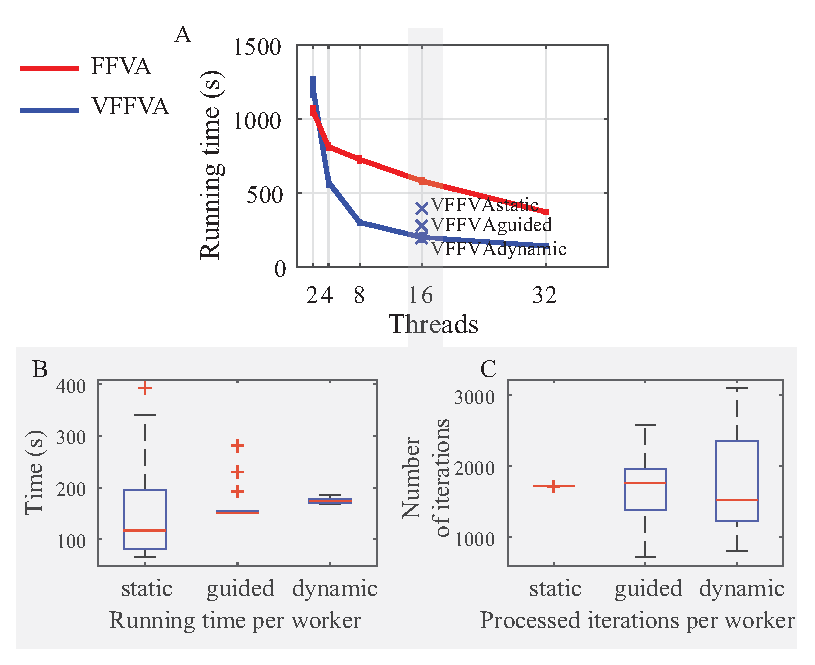
\includegraphics[width=\textwidth,height=7cm,keepaspectratio]{schedule.eps}
%\centerline{\includegraphics{fig01.eps}}
\caption[Run times of E\textsubscript{c} \textunderscore Matrix model.]{Run times of E\textsubscript{c} \textunderscore Matrix model. A-Run times of E\textsubscript{c} \textunderscore Matrix model at 2,4,8,16, and 32 threads using FFVA and VFFVA. B-Run time per worker in the static, guided, and dynamic schedule using 16 threads. C-The number of iterations processed per worker in the static, guided, and dynamic schedule using 16 threads.}\label{fig:static.}
\end{figure}
\noindent VFFVA offers two nested levels of parallelism. In shared memory systems, the Open Multi-Processing (OpenMP) (\citealp{dagum1998openmp}) library allows balancing the load among the threads dynamically such that every instruction runs for an equal amount of time. In systems that do not share memory, Message Passing Interface (MPI) (\citealp{message2012mpi}) was used to create instances of the metabolic model. Consequently, the shared memory balancing through OpenMP is executed within each process.\\
The hybrid MPI/OpenMP architecture of parallelism allows great flexibility of usage, particularly in High-Performance Computing (HPC) setting.

\section{Results}
VFFVA and FVA were compared on the \textit{E. coli} coupled expression and metabolism model (\citealp{thiele2009genome}) that has 13726 reactions using static, guided and dynamic load balancing strategies.
Using the static schedule, VFFVA assigned an equal number of iterations to every worker. With 16 threads, the number of iterations per worker equaled 1715 and 1716 (Figure \ref{fig:static.}-C). Expectedly, the run time varied widely between workers (Figure \ref{fig:static.}-B) and resulted in a final time of 393$s$. Another type of load balancing is the guided schedule which consists of dividing the reactions in chunks of size $reactions/workers$ initially and $remaining\textunderscore{reactions}/workers$ afterward. Using guided schedule (Figure \ref{fig:static.}-A), while the run time per worker was quite comparable with a final time of 281$s$, the reactions processed per worker varied between 719 and 2581.
Using a dynamic load balancing with a chunk size of 50 reactions resulted in a perfect synchronization between the workers and a final run time of 197$s$, while FFVA took 581$s$. An optimal reaction chunk size has to be small enough to ensure a frequent update on the workers' load, and big enough to take advantage of the solution basis reuse in every worker.\\ 
For ill-conditioned problems typically occurring during the generation of warmup points for the sampling of metabolic models, dynamic load balancing can reduce the run time by a factor of up to 100 (Supplementary Information). Additionally, VFFVA requires only the memory to load the metabolic model resulting in 14 fold decrease in memory usage (Supplementary Information). \\
Taken together, as metabolic models are steadily growing in number and complexity, their analysis requires the design of efficient tools. VFFVA allows making the most of modern machines specifications to run a more considerable amount of simulation in less time thereby enabling biological discovery. 

%\begin{figure}[!tpb]%figure2
%%\centerline{\includegraphics{fig02.eps}}
%\caption{Caption, caption.}\label{fig:02}
%\end{figure}

\section*{Acknowledgements}

The author would like to thank Valentin Plugaru at the University of Luxembourg for useful comments and guidance as well as fastFVA authors for publicly sharing their code and IBM for providing a free academic version of ILOG CPLEX. The experiments presented in this paper were partly carried out
using the HPC facilities of the University of Luxembourg~(\citealp{VBCG_HPCS14}).

\bibliographystyle{natbib}
%\bibliographystyle{achemnat}
%\bibliographystyle{plainnat}
%\bibliographystyle{abbrv}
%\bibliographystyle{bioinformatics}
%
%\bibliographystyle{plain}
%
\bibliography{references}


\end{document}
